\section{The isolated harmonic-layer obstruction}
\label{sec:rigidity}

For a nonempty spherical type, we prove that prescribed null-vector data
outside it force some capped representative to meet a closed layer bound
inside it.
This supplies the nonemptiness of the closed sublevels used when a harmonic
height comparison has a null-vector tie.  Throughout this section,
$E_L=E_L(x)=B_xP_{o,L}$ denotes the family from
Section~\ref{sec:height-data}, and $Y_L^d$ denotes its pure layer of level $d$.
We retain both the cochain and internal gradings.  All signs below are
cochain signs.

\begin{proposition}[Isolated harmonic layer]
\label{prop:isolated-layer}
Let $I\subseteq S$ be nonempty and connected.  Let $c_I$ be a strictly
positive vector with $C_Ic_I=0$, and extend $c$ by zero on
$\widehat S\setminus I$.  Let $J\subseteq I$ be spherical, possibly
empty, let $q>0$ be an integer, and fix a coset $A_Jx$.  Suppose that the
fixed data on $(I\setminus J)\cup\partial I$ are capped at $q$ and
satisfy
\begin{equation}
 m^q|_{(I\setminus J)\cup\partial I}
   =c|_{(I\setminus J)\cup\partial I}.
 \label{eq:rigidity-exterior-data}
\end{equation}
It is impossible that every representative $z\in A_Jx$ capped at $q$ on
$I$ satisfies
\begin{equation}
 m_j^q(z)>c_j\qquad\text{for every }j\in J.
 \label{eq:rigidity-strict-hypothesis}
\end{equation}
Equivalently, if $J\ne\varnothing$ and
\eqref{eq:rigidity-exterior-data} holds, there is a representative capped
on $I$ and a color $j\in J$ with $m_j^q\le c_j$.  If $J=\varnothing$,
the exterior situation \eqref{eq:rigidity-exterior-data} itself is
impossible.
\end{proposition}

The proof assumes the strict inequalities at every capped representative.
Convex subobjects turn this hypothesis into an ordinary interior condition
on the excess of the level-$q$ multiplicities over $c$.  We then remove
socles from successive lower layers by positive twists, preserving the cap
and the conditions already established.  The Hom estimates below justify
these moves and force each
processed layer to avoid $\partial I$.  Since the frame contributes at
level zero, some layer below $q$ meets $\partial I$, giving the
contradiction.

\subsection{Linear Hom complexes and their three-column filtration}

Let $P$ and $Y$ be pure projective layers of levels $l$ and $k$, respectively.
For $i\in\{0,1,2\}$, let
$\mathcal L_i^{n,v}(P,Y)$ be the space of maps of path length $i$, cochain
degree $n$, and internal degree $v$.  Such a space can be nonzero only if
\begin{equation}
 n+v=k-l+i.
 \label{eq:rigidity-hom-degree}
\end{equation}
Indeed, a path-length-$i$ map between generators at placements $(c,u)$
and $(c',u')$ has degrees $n=c'-c$ and $v=u'+i-u$.
Write $\delta_P$ and $\delta_Y$ for the linear differentials of the layers.
The linear Hom differential is
\[
 D_1f=\delta_Yf-(-1)^n f\delta_P:
 \mathcal L_i^{n,v}(P,Y)\longrightarrow
 \mathcal L_{i+1}^{n+1,v}(P,Y).
\]
Put
\[
 \mathsf H_i^{n,v}(P,Y)=
 \frac{\ker\bigl(D_1|_{\mathcal L_i^{n,v}(P,Y)}\bigr)}
 {\operatorname{im}\bigl(D_1|_{\mathcal L_{i-1}^{n-1,v}(P,Y)}\bigr)},
 \qquad
 h_i(P,Y)=\sum_{n,v}\dim_{\C}\mathsf H_i^{n,v}(P,Y),
\]
where a space with path length outside $\{0,1,2\}$ is zero.  These sums are
finite, and the dimensions in them are unsigned.  In particular,
$\mathsf H_0$ has no boundaries: it consists of the homogeneous maps of
coefficient arrays commuting with the linear differentials up to the
indicated cochain sign.  The image of such a map is a graded
subrepresentation, after accounting for its placements.

\begin{lemma}[Hom pairing and middle vanishing]
\label{lem:rigidity-hom-filtration}
For pure projective layers $P,Y$, including those formed from graded
subrepresentations, there are perfect pairings
\[
 \mathsf H_i^{n,v}(P,Y)\ \times\
 \mathsf H_{2-i}^{-n,\,2-v}(Y,P)\longrightarrow\C.
\]
Consequently,
\begin{equation}
 \begin{split}
 h_2(P,Y)&=h_0(Y,P),\\
 (\dim P)^{\mathsf t}\widetilde C\,\dim Y
   &=h_0(P,Y)+h_0(Y,P)-h_1(P,Y).
 \end{split}
 \label{eq:rigidity-euler}
\end{equation}
Here $\dim P$ and $\dim Y$ count projective generators, with all placements
included.  For any two labels $L,H$ and any levels $l,k$,
\begin{equation}
 h_1(Y_L^l,Y_H^k)=0.
 \label{eq:rigidity-middle-vanishing}
\end{equation}
The same vanishing holds after replacing either layer by a direct summand
as a pure layer.
\end{lemma}

\begin{proof}
The symmetric Frobenius trace of $Z$, normalized by
$\operatorname{tr}(\theta_\alpha)=1$, pairs paths of length $i$ perfectly
with opposite paths of length $2-i$.  On complexes use the supertrace
\[
 \operatorname{Str}_Y(a)
   =\sum_c(-1)^c\operatorname{tr}(a|_{Y^c}).
\]
Here $Y^c$ denotes the cochain-degree-$c$ term, and the trace includes
the ordinary matrix trace on multiplicity spaces.  The
summandwise pairing
$\langle f,g\rangle=\operatorname{Str}_Y(f\circ g)$ is perfect between
$\mathcal L_i^{n,v}(P,Y)$ and
$\mathcal L_{2-i}^{-n,2-v}(Y,P)$.  Cyclicity gives, for the complementary
degrees appearing in a differential pairing,
\[
 \langle D_1f,g\rangle+(-1)^n\langle f,D_1g\rangle=0.
\]
There is no sign from the internal degree.  Finite-dimensional duality
therefore gives the asserted perfect pairings on cohomology.  This
argument uses only the linear differentials and the Frobenius pairing,
so it also applies to the pure layers associated with graded
subrepresentations.

The alternating sum of the dimensions of the three path-length columns
is $(\dim P)^{\mathsf t}\widetilde C\dim Y$: there are two equal-vertex
paths, of lengths zero and two, and the length-one paths contribute the
negative adjacency entries.  Euler characteristic and the pairing of
columns zero and two give \eqref{eq:rigidity-euler}.

For the remaining assertion, consider the full bigraded Hom complex
$\Hom_Z(E_L,E_H)$.  Minimality writes each projective differential as a
sum of its length-one and length-two parts.  Thus its Hom differential is
$D_1+D_2$, where $D_a$ raises path length by $a$.  Filter Hom by paths of
length at least $i$.  There are only the three columns $0,1,2$; the first
nonzero differential is $D_1$.  Its cohomology decomposes as the direct
sum of the spaces above, indexed by the ordered pair of source and target
layers.  After this page, the only possible differential goes from column
zero to column two.  Every column-one class is therefore permanent.

By Proposition~\ref{prop:twist-action}, applying $B_x$ preserves the
bigraded Hom cohomology.  Between the initial frame projectives this
cohomology is zero when $L\ne H$.  When $L=H$, it has dimension one in each
of bidegrees $(0,0)$ and $(0,2)$ and is zero elsewhere.  Both of these
dimensions have specific permanent representatives in the filtration.
First, the identity of $E_L$ is a nonzero class in column zero and bidegree
$(0,0)$; a boundary cannot have a length-zero component.  Second, choose
one projective summand in the nonzero minimal complex $E_L$, and place its
normalized token on that diagonal matrix entry, with all other entries
zero.  This is a cycle in bidegree $(0,2)$, since a token multiplied on
either side by a radical entry is zero.  If the chosen summand is in
cochain placement $c$, this cycle has supertrace $(-1)^c\ne0$.
Every Hom boundary has zero supertrace by graded cyclicity, so the token
cycle is nonzero in actual Hom cohomology.  It lies in filtration two,
and filtration three is zero; hence it supplies a nonzero column-two
class in the associated graded cohomology.

The identity and token exhaust the two actual diagonal Hom dimensions.
All actual off-diagonal Hom cohomology vanishes.  Since every column-one
class is permanent, every such class must be zero, proving
\eqref{eq:rigidity-middle-vanishing}.  Finally, a direct summand of a pure
layer gives a direct summand of each linear Hom complex.  Its column-one
cohomology is therefore zero as well.  This last argument is on the
linear page; it does not assert that the chosen layer summand splits off
from the full complex $E_L$.
\end{proof}

The numerical identity \eqref{eq:rigidity-euler} parallels
Crawley--Boevey's Hom--Ext formula for preprojective modules
\cite[Lemma~1]{CrawleyBoevey2000}.

We will also use weighted versions of these formulas.  For families
$\mathcal P=(P_L)_L$ and $\mathcal Y=(Y_H)_H$, define the nonnegative real
number
\[
 h_i^{\mathrm{wt}}(\mathcal P,\mathcal Y)
   =\sum_{L,H}w_Lw_H h_i(P_L,Y_H).
\]
These are weighted dimensions, not necessarily integer dimensions of
vector spaces.  If the two weighted generator arrays are $\phi p$ and
$\phi y$, respectively, then
\[
 \sum_{L,H}w_Lw_H
 (\dim P_L)^{\mathsf t}\widetilde C\dim Y_H
   =(\phi p)^{\mathsf t}\widetilde C\phi y
   =D_0p^{\mathsf t}Cy,
 \qquad D_0=\sum_Lw_L^2.
\]
The symmetry of $w_Lw_H$ under interchange of the labels gives
\begin{equation}
 D_0p^{\mathsf t}Cy
   =h_0^{\mathrm{wt}}(\mathcal P,\mathcal Y)
    +h_0^{\mathrm{wt}}(\mathcal Y,\mathcal P)
    -h_1^{\mathrm{wt}}(\mathcal P,\mathcal Y).
 \label{eq:rigidity-weighted-euler}
\end{equation}

\begin{lemma}[The capped secondary injection]
\label{lem:rigidity-secondary-injection}
Let $I\subseteq S$, and suppose the family $E_L$ is capped at $q$ on $I$.
For every $L$, let $M_L$ be a direct summand of the pure layer $Y_L^q$
supported on $\widetilde I$.  If $d<q$, then for every pair of labels $L,H$
there are injections
\begin{equation}
 \mathsf H_0^{n,v}(M_L,Y_H^d)
   \lhook\joinrel\longrightarrow
 \mathsf H_2^{n+1,v}(M_L,Y_H^{d-1}),
 \qquad n+v=d-q.
 \label{eq:rigidity-secondary-injection}
\end{equation}
In particular, for $\mathcal M=(M_L)_L$ and
$\mathcal Y^d=(Y_H^d)_H$,
\begin{equation}
 h_0^{\mathrm{wt}}(\mathcal M,\mathcal Y^d)
 \le h_0^{\mathrm{wt}}(\mathcal Y^{d-1},\mathcal M).
 \label{eq:rigidity-secondary-bound}
\end{equation}
\end{lemma}

\begin{proof}
Represent a class on the left of
\eqref{eq:rigidity-secondary-injection} by a homogeneous length-zero
linear cocycle $f$, and extend it by zero on the other source-layer
summands.  This is a linear cocycle in $\Hom_Z(E_L,E_H)$ because $M_L$ is
a direct summand for the linear differential.  It defines an embedded
column-zero class on the page after $D_1$: the linear differential
preserves the ordered source/target layer pair, and column zero has no
incoming boundaries.

Write the length-two projective differentials as $d_{E_L}^{(2)}$ and
$d_{E_H}^{(2)}$.  The secondary differential on this class is represented
by
\[
 d_{E_H}^{(2)}f-(-1)^n f d_{E_L}^{(2)}.
\]
The only possible ordered layer pairs in its target are
\begin{equation}
 \begin{array}{ccl}
 (q,d-1)&\text{from}&d_{E_H}^{(2)}f,\\
 (q+1,d)&\text{from}&f d_{E_L}^{(2)}.
 \end{array}
 \label{eq:rigidity-secondary-blocks}
\end{equation}
A length-two entry is diagonal in the unfolded vertex and lowers the
layer by one.  For the second term in
\eqref{eq:rigidity-secondary-blocks} to be nonzero, its source would have
to lie at level $q+1$ on a vertex of $\widetilde I$.  Such generators are
excluded by the cap.  Vertices outside $\widetilde I$ cannot contribute
through a diagonal length-two entry.  Thus the secondary image lies
entirely in the first block.  The splitting $Y_L^q=M_L\oplus M_L^{\prime}$
is a splitting for the linear differential, so it splits the target
column-two cohomology by source summands as well.  The target-side
composite is zero on $M_L^{\prime}$ and therefore lands in the summand
$\mathsf H_2(M_L,Y_H^{d-1})$, giving the map in
\eqref{eq:rigidity-secondary-injection}.

If a class were in its kernel, it would be permanent: no differential
enters column zero, and there is no possible differential after the
secondary one.  Its total degree is $d-q<0$.  Actual Hom cohomology between
$E_L$ and $E_H$ is zero in this degree by the computation in
Lemma~\ref{lem:rigidity-hom-filtration}.  The class is therefore zero.
This proves the injection for each pair of labels before any weighting.
Sum the resulting dimension inequalities with positive weights $w_Lw_H$
and use the dual pairing of
Lemma~\ref{lem:rigidity-hom-filtration}; the result is
\eqref{eq:rigidity-secondary-bound}.
\end{proof}

Figure~\ref{fig:hom-filtration} records the two possible secondary
targets.  The tensor estimate in Figure~\ref{fig:filtrations} excluded
an incoming secondary differential at a maximal pair of levels.  Here the
cap removes one outgoing term, so negative-degree Hom vanishing forces
injection into the other target.

\begin{figure}[tbp]
  \centering
  {\small
    Linear part: $C_0\xrightarrow{d_1}C_1\xrightarrow{d_1}C_2$,
    \quad $H_a=H^a(C_\bullet,d_1)$.\par}
  \medskip
  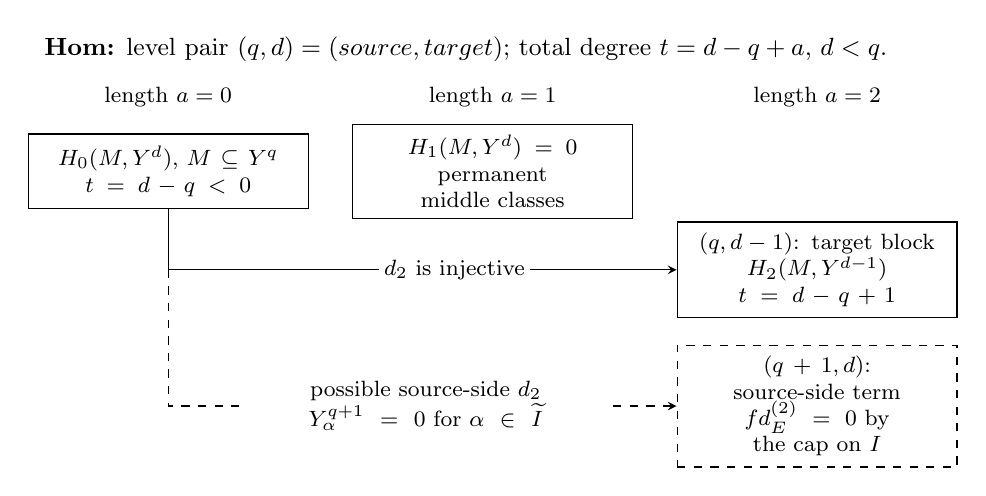
\begin{tikzpicture}[
      x=.01\linewidth,y=1cm,
      every node/.style={font=\footnotesize,align=center},
      term/.style={text width=.27\linewidth,inner sep=4pt},
      permanent/.style={term,draw,semithick,minimum height=.95cm},
      endpoint/.style={term,draw,thin,minimum height=.95cm},
      excluded/.style={term,draw,dashed,thin,minimum height=.95cm},
      differential/.style={->,thin,>=stealth}
    ]
    \node[anchor=west,align=left,font=\small] at (-14,-4.55)
      {\textbf{Hom:} level pair $(q,d)=(\text{source},\text{target})$;
        total degree $t=d-q+a$, $d<q$.};
    \node at (0,-5.16) {length $a=0$};
    \node at (34,-5.16) {length $a=1$};
    \node at (68,-5.16) {length $a=2$};
    \node[endpoint] (hom-zero) at (0,-6.1)
      {$H_0(M,Y^d)$, $M\subseteq Y^q$\\$t=d-q<0$};
    \node[permanent] (hom-middle) at (34,-6.1)
      {$H_1(M,Y^d)=0$\\permanent middle classes};
    \node[endpoint] (hom-target) at (68,-7.35)
      {$(q,d-1)$: target block\\$H_2(M,Y^{d-1})$\\$t=d-q+1$};
    \node[excluded] (hom-source) at (68,-9.08)
      {$(q+1,d)$: source-side term\\$f d_E^{(2)}=0$ by the cap on $I$};
    \draw[differential] (hom-zero.south) -- (0,-7.35)
      -- (hom-target.west);
    \node[fill=white,inner sep=2pt] at (30,-7.35)
      {$d_2$ is injective};
    \draw[differential,dashed] (0,-7.35) -- (0,-9.08)
      -- (hom-source.west);
    \node[fill=white,text width=.38\linewidth,inner sep=2pt] at (27,-9.08)
      {possible source-side $d_2$\\
        $Y^{q+1}_\alpha=0$ for $\alpha\in\widetilde I$};
  \end{tikzpicture}
  \caption{The Hom length filtration for a direct summand $M$ of $Y^q$
    supported on $\widetilde I$, with the family capped at $q$ on $I$.
    Here $d<q$, and $H_a$ denotes the linear cohomology $\mathsf H_a$ with
    family and bidegree indices suppressed.  The secondary differential
    of a length-zero linear cocycle $f$ has the two displayed target blocks;
    $d_E^{(2)}$ denotes the length-two part of the source differential.
    The source-side contribution
    $f d_E^{(2)}$ vanishes: length-two paths are diagonal and the cap
    excludes level-$q+1$ source generators on $\widetilde I$.
    Higher source generators outside $I$ need not vanish.
    Negative-degree actual Hom vanishes, forcing injection into the
    remaining target block.  The identity and token classes give the
    middle vanishing proved in Lemma~\ref{lem:rigidity-hom-filtration}.
    The dashed arrow marks an excluded possibility.}
  \label{fig:hom-filtration}
\end{figure}


\subsection{Convex subrepresentations and the boundary sign}

The following consequence of the Hom calculation isolates the convex
part of the argument.  For a family of layers, saying that its socle
vanishes on a color set means that this holds at every unfolded vertex
of those colors in every member of the family.

\begin{lemma}[Separation from the boundary]
\label{lem:rigidity-separation}
Let $I\subseteq S$ be nonempty and connected, and let $c$ be zero off $I$
and strictly positive on $I$, with $C_Ic_I=0$.  Let $J\subseteq I$.
Suppose $\mathcal M=(M_L)_L$ is a family of direct summands of one pure
layer of the family $E_L$, supported on $\widetilde I$, with weighted
generator array $\phi m$.  Assume $m-c$ is supported on $J$ and that
$(m-c)_J$ is an interior point in $\R^J$ of the convex hull of finitely
many vectors $s_J$ with the following properties: $s$ is zero off $J$,
and $\phi s$ is the weighted generator array of a family of graded
subrepresentations $\mathcal S=(S_L)_L\subseteq\mathcal M$ supported on
$\widetilde J$.

Let $\mathcal Y=\mathcal Y^d$ be any layer of the family $E_L$, and write
$\phi y$ for its weighted generator array.  If its socle vanishes on $J$,
then
\begin{equation}
 y|_{\partial I}=0,\qquad
 (Cy)_J=0,\qquad
 h_0^{\mathrm{wt}}(\mathcal M,\mathcal Y)
 =h_0^{\mathrm{wt}}(\mathcal Y,\mathcal M)=0.
 \label{eq:rigidity-separation-conclusions}
\end{equation}
Here $\partial I$ is the outside-neighbor set, including the frame.
The assertion includes the usual interior convention in $\R^0$ when
$J=\varnothing$.
\end{lemma}

\begin{proof}
Fix one of the subrepresentation families $\mathcal S$.  A nonzero
homogeneous coefficient-array map $S_L\to Y_H$ has a nonzero graded
image supported on $\widetilde J$.  Such an image has a socle: arrow
coefficients raise cochain placement, so a nonzero coefficient in its
highest occupied placement is killed by every outgoing arrow.  Since
the image is a subrepresentation, this is a socle of $Y_H$ on
$\widetilde J$.  The hypothesis therefore gives
\[
 h_0^{\mathrm{wt}}(\mathcal S,\mathcal Y)=0.
\]
Also, composition with the inclusion $S_L\hookrightarrow M_L$ gives
injections on length-zero linear cocycles, with no length-zero
boundaries to quotient out.  Thus
\[
 h_0^{\mathrm{wt}}(\mathcal Y,\mathcal S)
 \le h_0^{\mathrm{wt}}(\mathcal Y,\mathcal M).
\]
Apply \eqref{eq:rigidity-weighted-euler} first to
$(\mathcal S,\mathcal Y)$ and then to $(\mathcal M,\mathcal Y)$.
The first application uses only
$h_1^{\mathrm{wt}}(\mathcal S,\mathcal Y)\ge0$; the second has
$h_1^{\mathrm{wt}}(\mathcal M,\mathcal Y)=0$ by
Lemma~\ref{lem:rigidity-hom-filtration}.  Subtracting gives
\begin{equation}
 D_0(m-s)^{\mathsf t}Cy
 \ge h_0^{\mathrm{wt}}(\mathcal M,\mathcal Y)\ge0.
 \label{eq:rigidity-convex-inequality}
\end{equation}
In particular, no middle-Hom vanishing for $\mathcal S$ is required.

The left side of \eqref{eq:rigidity-convex-inequality} is affine-linear
in $s$, so the inequality holds throughout the convex hull.  At its
interior point $e=m-c$, it gives
\begin{equation}
 D_0c^{\mathsf t}Cy
 \ge h_0^{\mathrm{wt}}(\mathcal M,\mathcal Y)\ge0.
 \label{eq:rigidity-null-average}
\end{equation}
On the other hand, symmetry of $C$, the null equation on $I$, and
nonnegativity of $y$ give
\begin{equation}
 c^{\mathsf t}Cy
  =-\sum_{a\notin I}\sum_{i\in I}b_{ai}c_i y_a\le0.
 \label{eq:rigidity-boundary-sign}
\end{equation}
This is strictly negative if $y_a>0$ for any $a\in\partial I$.
Consequently $y|_{\partial I}=0$, the two sides of
\eqref{eq:rigidity-null-average} are zero, and
$h_0^{\mathrm{wt}}(\mathcal M,\mathcal Y)=0$.

Because $e_J$ is an ordinary real interior point, for each $j\in J$ the
hull contains $e_J\pm\varepsilon\mathbf e_j$ for sufficiently small
$\varepsilon>0$.  Substituting these two points into
\eqref{eq:rigidity-convex-inequality}, whose value at $e$ is now zero,
forces $(Cy)_j=0$.  It follows that
\[
 m^{\mathsf t}Cy
   =c^{\mathsf t}Cy+(m-c)_J^{\mathsf t}(Cy)_J=0.
\]
The weighted Euler identity, with middle vanishing for $\mathcal M$,
now forces $h_0^{\mathrm{wt}}(\mathcal Y,\mathcal M)=0$ as well.
When $J=\varnothing$, one has $m=c$ and the hull is the singleton in
$\R^0$; the same argument applies with no coordinate perturbations.
\end{proof}

\subsection{The socle-removal induction}

\begin{proof}[Proof of Proposition~\ref{prop:isolated-layer}]
Assume \eqref{eq:rigidity-strict-hypothesis} holds at every capped
representative.  Since
$\partial J\subseteq(I\setminus J)\cup\partial I$,
Lemma~\ref{lem:cap-accessibility} supplies a representative capped on $J$
and hence on all of $I$.  We shall move only among such representatives.
All the exterior data in \eqref{eq:rigidity-exterior-data} stay fixed,
since operations in $A_J$ change multiplicities only in colors of $J$.

At any capped representative, let $M_L$ be the part of $Y_L^q$ supported
on $\widetilde I$, and set $\mathcal M=(M_L)_L$.  This is a direct
summand of the pure layer: its outside neighbors have zero multiplicity
at level $q$ by \eqref{eq:rigidity-exterior-data}, so no linear arrow
joins it to the rest of that layer.  This statement concerns the pure
layer, and does not assert a splitting of $E_L$.  By
Lemma~\ref{lem:family-proportionality}, its weighted generator array is
$\phi m$, where $m$ equals $m^q$ on $I$ and is zero off $I$.

Harmonizing the full level-$q$ vector on $J$ gives the coordinates $c_J$.
Indeed, only neighbors of $J$ enter these equations, their prescribed
values are those of $c$, and $C_Ic_I=0$; uniqueness follows from the
sphericity of $J$.  Remote coordinates outside $I\cup\partial I$ do not
enter these equations.  Capping a representative on $J$, with the fixed
exterior cap, is equivalent to capping it on $I$.
Proposition~\ref{prop:convex-subobjects} therefore applies with its strict,
universally quantified hypothesis.  It shows that
\begin{equation}
 e=m-c,\qquad \supp(e)\subseteq J,
 \qquad
 e_J\in\operatorname{int}_{\R^J}
 \operatorname{conv}\{s_J\},
 \label{eq:rigidity-interior}
\end{equation}
where each $s$ is the folded weighted dimension of subrepresentations
$\mathcal S\subseteq\mathcal M$ supported on $\widetilde J$.
Such subrepresentations, initially obtained in the full layer, lie in
$\mathcal M$ because of their support.

The interior in \eqref{eq:rigidity-interior} is the ordinary real
interior supplied by Proposition~\ref{prop:convex-subobjects}, even when
folded multiplicities are not integers.  For $J=\varnothing$, it means
$e=0$ in $\R^0$.

Thus Lemma~\ref{lem:rigidity-separation} applies at every capped
representative.  This uniformity is essential: both $\mathcal M$ and its
convex hull may change during the following operations, but the
hypothesis \eqref{eq:rigidity-strict-hypothesis} supplies
\eqref{eq:rigidity-interior} anew after each cap-preserving move.

Let $d_b$ be the lowest layer that meets $\partial I$.  This level exists
because the frame $o$ belongs to $\partial I$ and $m_o^0=1$.  It is fixed
throughout the coset, and
\begin{equation}
 d_b\le0<q.
 \label{eq:rigidity-boundary-level}
\end{equation}
Choose an integer $d_{\min}$ below or equal to every initially occupied
layer of every member of the family.  Positive operations cannot create
layers below $d_{\min}$ by their amplitude.  We shall proceed through
$d=d_{\min},\ldots,d_b$.  At the beginning of a stage, the induction
conditions are, for every $k<d$,
\begin{equation}
 \begin{aligned}
 \operatorname{soc}_{\widetilde J}\mathcal Y^k&=0,
 & (Cm^k)_J&=0,\\
 h_0^{\mathrm{wt}}(\mathcal Y^k,\mathcal M)&=0,
 & h_0^{\mathrm{wt}}(\mathcal M,\mathcal Y^k)&=0.
 \end{aligned}
 \label{eq:rigidity-induction}
\end{equation}
Here $m^k$ is the folded vector of the full layer $\mathcal Y^k$, and
$\mathcal M$ always denotes the current level-$q$ summand.  The conditions
hold initially since all lower layers are zero.

Since $d\le d_b<q$, Lemma~\ref{lem:rigidity-secondary-injection} and the
condition at $d-1$ give
\begin{equation}
 h_0^{\mathrm{wt}}(\mathcal M,\mathcal Y^d)=0.
 \label{eq:rigidity-current-hom-zero}
\end{equation}
Suppose that $\mathcal Y^d$ has a nonzero socle in a color $j\in J$.
Then $\mathcal M$ has zero top in that color.  To see this, a top simple
quotient of some $M_L$ and a socle simple of some $Y_H^d$ at the same
unfolded vertex compose to a nonzero homogeneous length-zero map.
Lemma~\ref{lem:family-proportionality} ensures that if a top occurs
anywhere in color $j$ in the family, then it occurs at every label in
that color in some family member.  It can therefore be matched with the
label of the chosen socle.  The resulting map would contradict
\eqref{eq:rigidity-current-hom-zero}, since every weight is positive.

Apply $F_j$ to this representative.  The top of $\mathcal M$ at color
$j$ is the top of the full level-$q$ layer there, because $\mathcal M$ is
a direct summand containing that color.  Its vanishing makes this move
cap-preserving by Lemma~\ref{lem:cap-accessibility}.  Concretely, the only
new level-$q+1$ contribution from the level-$q$ layer is this top; higher
layers have no generators on $I\cup\partial I$, and the twist acts
identically on that remote part.  Other colors keep their multiplicities.

We next prove that this move preserves
\eqref{eq:rigidity-induction} and changes the level-$d$ layer only by its
unshifted positive operation.  Denote the data immediately before and
after the move by ``old'' and ``new''.  For this single move, ascend again
through the integers $k<d$, starting below all occupied layers.  Suppose
that the old top at color $j$ in level $k-1$ has already been shown to
vanish.  This is vacuous at the starting level.
Lemma~\ref{lem:layers-amplitude-extension} then identifies
\begin{equation}
 \mathcal Y^k_{\mathrm{new}}
   \cong\text{the level-$k$ part of }F_j\mathcal Y^k_{\mathrm{old}}.
 \label{eq:rigidity-unshifted-step}
\end{equation}
Indeed, the level-$k$ term from the old level $k-1$ is exactly its top in
color $j$, and no other input layer contributes at $k$.  By
Lemma~\ref{lem:positive-layer}, the vanishing of the old socle on $J$
implies the vanishing of the new socle on $J$ in
\eqref{eq:rigidity-unshifted-step}.

The new representative is capped, so
Lemma~\ref{lem:rigidity-separation} applies using its new family
$\mathcal M_{\mathrm{new}}$.  As $k<d\le d_b$, the layer has no boundary
support.  The lemma yields all the new conditions
\eqref{eq:rigidity-induction} at this $k$, including
$(Cm^k_{\mathrm{new}})_j=0$.  The old row is also zero, and all
multiplicities off color $j$ are unchanged.  Since $C_{jj}=2$, comparison
of the two rows gives
\[
 2\bigl(m^k_{\mathrm{new},j}-m^k_{\mathrm{old},j}\bigr)=0.
\]
Let $t_j^k\ge0$ be the folded weighted top multiplicity of
$\mathcal Y^k_{\mathrm{old}}$ in color $j$.  Formula
\eqref{eq:layers-positive-dimension}, together with
\eqref{eq:rigidity-unshifted-step}, says
\[
 m^k_{\mathrm{new},j}
   =m^k_{\mathrm{old},j}-(Cm^k_{\mathrm{old}})_j+t_j^k.
\]
Thus $t_j^k=0$.  Positivity of the weights makes every old top in this
color zero, providing the premise at $k+1$.  This completes the upward
verification.  In particular, the old top at level $d-1$ is zero, so
\eqref{eq:rigidity-unshifted-step} also holds at $k=d$.

The order of this verification is important: the absence of a shifted-in
contribution at $k$ uses the top vanishing already established at $k-1$;
the top vanishing at $k$ is then deduced from the new row equation and the
pure-layer dimension formula.  Hence no assertion about the level being
checked is assumed in advance.  The verification also proves that
\eqref{eq:rigidity-current-hom-zero} can be used again after the move,
with the new $\mathcal M$, by
Lemma~\ref{lem:rigidity-secondary-injection}.

Continue applying $F_j$ whenever a socle in a color $j\in J$ remains in
level $d$.  This process terminates.  To prove it, consider only the
unshifted operations on that fixed pure layer.  By
Lemma~\ref{lem:layers-bottom-composition}, a composite is the bottom
cohomology of the corresponding positive word, so these operations
satisfy the positive braid relations.  A last-action color has zero
socle after its operation by Lemma~\ref{lem:positive-layer}.
Inductively suppose the colors used so far form a reduced expression
for $w\in W_J$, with the most recent operation written on the left.  If
the next chosen color $j$ were a left descent of $w$, a reduced
expression for $w$ would begin with $j$.  Braid moves would therefore
express the current pure layer as the result of an unshifted $F_j$
operation acting last.  Its socle in color $j$ would be zero,
contradicting the choice of $j$.  Each choice is consequently a Coxeter
ascent.  Since $W_J$ is finite, the number of choices at level $d$ is
bounded by the length of its longest element.

At termination, the socle on $J$ vanishes in the current layer $d$.
If $d<d_b$, Lemma~\ref{lem:rigidity-separation} supplies
\eqref{eq:rigidity-induction} also at $k=d$, and we proceed to the next
level.  The range from $d_{\min}$ to $d_b$ is finite, and the earlier
conditions were preserved during every move.  At $d=d_b$, the same
lemma asserts that the layer has no support on $\partial I$, contradicting
the definition of $d_b$.

If $J=\varnothing$, the procedure contains no firing steps: the socle
condition on $J$ is vacuous, \eqref{eq:rigidity-interior} says $m=c$, and
Lemma~\ref{lem:rigidity-separation} already contradicts the boundary
layer.  Thus the dimension-zero case is included.  The contradiction
proves the proposition.
\end{proof}
